\documentclass{article}

\usepackage[a4paper, total={6in, 8in}]{geometry}

\usepackage{amsmath}
\usepackage{amsfonts}
\usepackage{amssymb}
\usepackage[T1, T2A]{fontenc}
\usepackage[utf8]{inputenc}
\usepackage[english, russian]{babel}
\usepackage{graphics}
\usepackage{graphicx}

\geometry{
 a4paper,
 total={170mm,257mm},
 left=20mm,
 top=20mm,
 }

\author{Александр Валентинов}
\title{Лабораторная работа 3.6.1}

\begin{document}
   \subsection*{Работа 3.6.1}
   \section*{Спектральный анализ электрических сигналов}
   
   \paragraph{Цель работы:} изучение состава периодических электрических сигналов.
   
   \paragraph{В работе используются:} анализатор спектра, генератор прямоугольных импульсов, генератор сигналов специальной формы, осциллограф.
   
   \subsubsection*{Экспериментальная установка:}
   
   \begin{figure}[h]
   \centering
   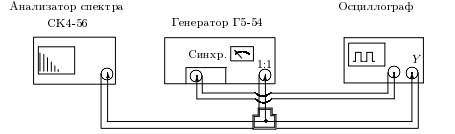
\includegraphics[width=10cm]{3_6_1a.jpg} 
   \caption{Схема для исследовния спектра периодической последовательности прямоугольных импульсов} 
   \label{fig.1} 
   \end{figure}
   
   \begin{figure}[h]
   \centering
   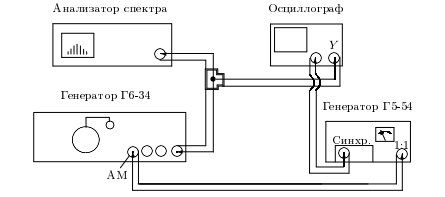
\includegraphics[width=10cm]{3_6_1b.jpg} 
   \caption{Схема для исследования спектра периодической последовательности цугов высокочастотных колебаний} 
   \label{fig.2} 
   \end{figure}

   \begin{figure}[h]
   \centering
   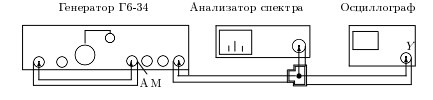
\includegraphics[width=10cm]{3_6_1c.jpg} 
   \caption{Схема для исследования спектра высокочастотного гармонического сигнала, промодулированного по амплитуде низкочастотным гармоничесим сигналом} 
   \label{fig.3} 
   \end{figure}

   \subsection*{Исследование спектра периодической последовательности прямоугольных импульсов}
   При длительности импульсов $\tau$ вдовое, $\Delta \nu$ уменьшается, а $\delta \nu$ остается прежней. При увеличении вдвое частоты повторения $f$, $\delta \nu$ увеличивается, а $\Delta \nu$ не изменяется. Качественная картина: рис. \ref{fig.a01} - \ref{fig.a03}. Количественные данные: табл. \ref{Ddtf}
   \begin{figure}[h!]
   \begin{minipage}[h!]{0.49\linewidth}
   \centering
   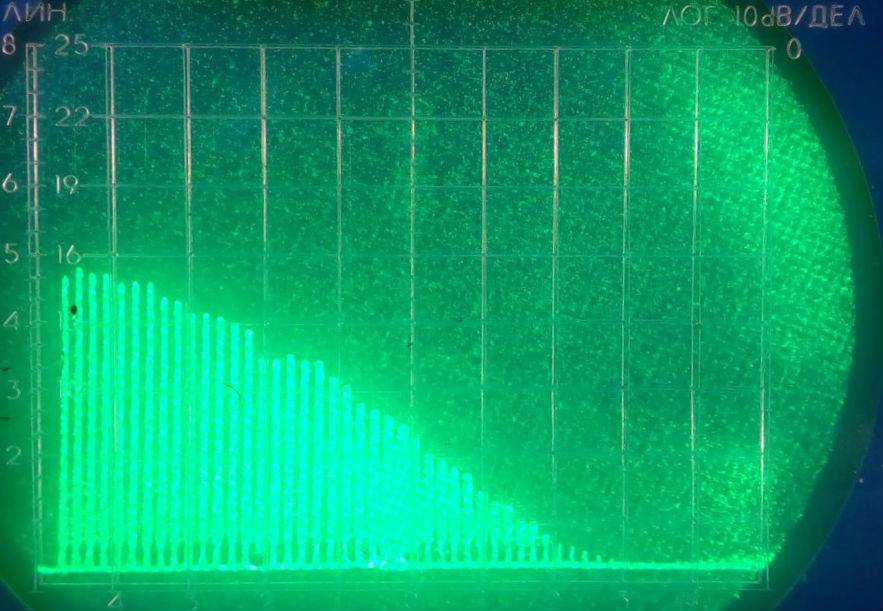
\includegraphics[height=4cm]{A01.jpg} 
   \caption{$f_{\text{повт}} = 1 \text{кГц},~ \tau = 25 \text{мкс}$} 
   \label{fig.a01} 
   \end{minipage}
   \hfill
   \begin{minipage}[h!]{0.49\linewidth}
   \centering
   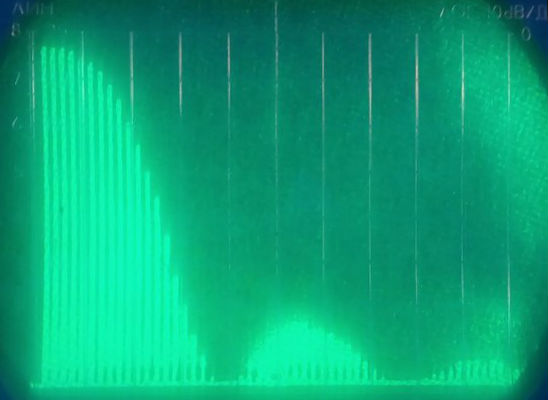
\includegraphics[height=4cm]{A02.jpg} 
   \caption{$f_{\text{повт}} = 1 \text{кГц},~ \tau = 50 \text{мкс}$} 
   \label{fig.a02}
   \end{minipage}
   \hfill
   \begin{minipage}[h!]{0.49\linewidth}
   \centering
   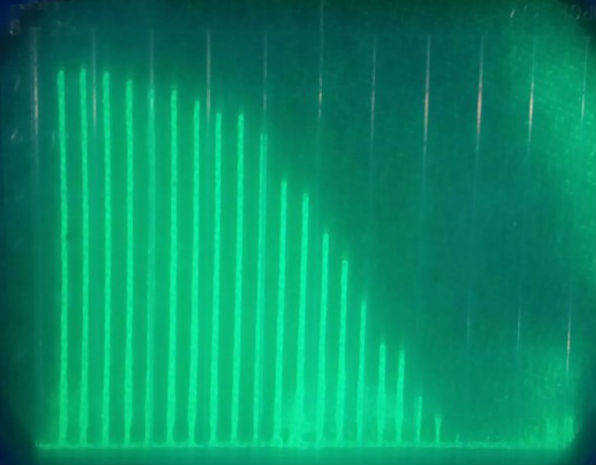
\includegraphics[height=4cm]{A03.jpg} 
   \caption{$f_{\text{повт}} = 2 \text{кГц},~ \tau = 25 \text{мкс}$} 
   \label{fig.a03}
   \end{minipage}
   \hfill
   \begin{minipage}[h!]{0.49\linewidth}
   \centering
   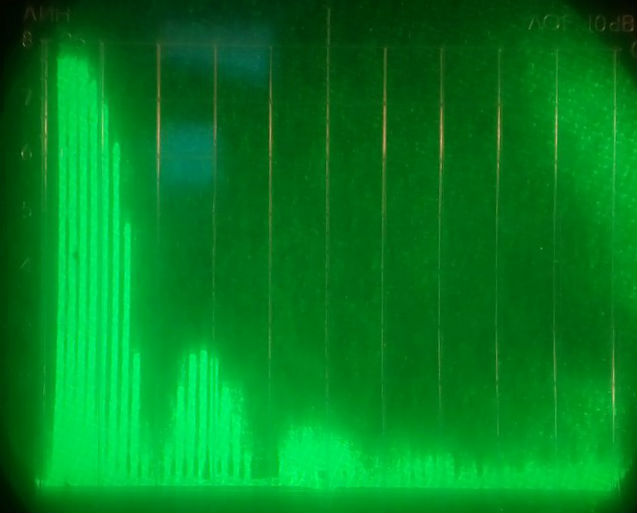
\includegraphics[height=4cm]{A04.jpg} 
   \caption{$f_{\text{повт}} = 1 \text{кГц},~ \tau = 100 \text{мкс}$} 
   \label{fig.a04}
   \end{minipage}  
   \end{figure}

   Для проверки соотношения неопределенности $\Delta\nu \Delta\tau \sim 1$ построим график $\Delta\nu(\tau^{-1})$ (Данные - табл. \ref{undefined}, график рис. \ref{fig.4})

   $$ \Delta \nu \Delta \tau \sim 1.06 \pm 0.06 $$

   Коэффициент графика сходится с единицой в пределах погрешности.

   \begin{table}[h!]
   \begin{center}
   \caption{Изменение $\Delta \nu$ и $\delta \nu$ при изменении $\tau$ и $f$}
   \label{Ddtf}
   \begin{tabular}{|*{6}{c|}}
   \hline 
   $f$, кГц & $\tau$, мкс & $\delta \nu$, кГц & $\Delta \nu$, кГц \\ \hline 
   1 & 25 & 1.00 & 40 \\ \hline 
   1 & 50 & 0.94 & 20 \\ \hline 
   2 & 25 & 2.06 & 40 \\ \hline 
   \end{tabular}
   \end{center} 
   \end{table}

   \begin{table}[h!]
   \begin{center}
   \label{undefined}
   \caption{Зависимость $\Delta(\tau^{-1})$}
   \begin{tabular}{|*{5}{c|}}
   \hline 
   $\tau$, мкс & $\tau^{-1}$, $\text{мкс}^{-1}$ & $\sigma_{\tau^{-1}}$, $\text{мкс}^{-1}$ & $\Delta \nu$, кГц & $\sigma_{\Delta \nu}$, кГц \\ \hline 
   25 & 4.00e-02 & 2e-03 & 40 & 3 \\ \hline 
   50 & 2.00e-02 & 4e-04 & 20 & 3 \\ \hline 
   80 & 1.25e-02 & 2e-04 & 10 & 3 \\ \hline 
   100 & 1.00e-02 & 1e-04 & 10 & 3 \\ \hline 
   140 & 7.14e-03 & 5e-05 & 7.1 & 0.7 \\ \hline 
   160 & 6.25e-03 & 4e-05 & 5.8 & 0.8 \\ \hline 
   200 & 5.00e-03 & 3e-05 & 1.7 & 0.8 \\ \hline 
   \end{tabular}
   \end{center} 
   \end{table} 

   \begin{figure}[h!]
   \centering
   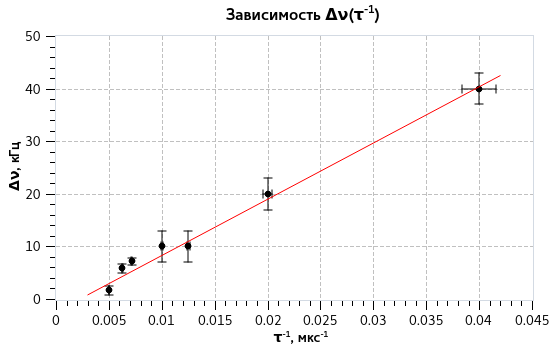
\includegraphics[width=10cm]{fig4.png} 
   \caption{Зависимость $\Delta \nu(\tau^{-1})$} 
   \label{fig.4} 
   \end{figure}
   
   \subsection*{Исследование спектра периодичексой последовтельности цугов гармонических колебаний}
   Для проверки соотнощения неопределенности построим график $\delta \nu(\nu_0)$:
   $$ \frac{d\delta \nu_0}{df} \sim 0.93 \pm 0.08 $$
   Соотношение сходится с единицей в пределах погрешности. 

   \begin{figure}[h!]
   \begin{minipage}[h!]{0.49\linewidth}
   \centering
   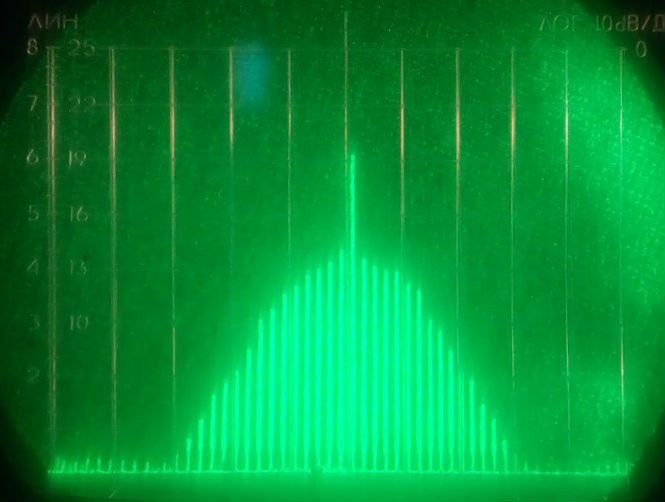
\includegraphics[height=4cm]{B01.jpg} 
   \caption{$f_{\text{повт}} = 1 \text{кГц},~ \tau = 50 \text{мкс},~ f_{0} = 25 \text{кГц}$} 
   \label{fig.b01} 
   \end{minipage}
   \hfill
   \begin{minipage}[h!]{0.49\linewidth}
   \centering
   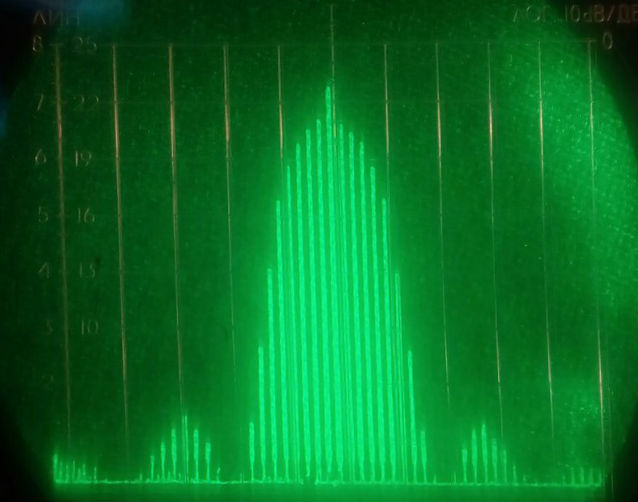
\includegraphics[height=4cm]{B02.jpg} 
   \caption{$f_{\text{повт}} = 1 \text{кГц},~ \tau = 100 \text{мкс},~ f_{0} = 25 \text{кГц}$} 
   \label{fig.b02}
   \end{minipage}
   \hfill
   \begin{minipage}[h!]{0.49\linewidth}
   \centering
   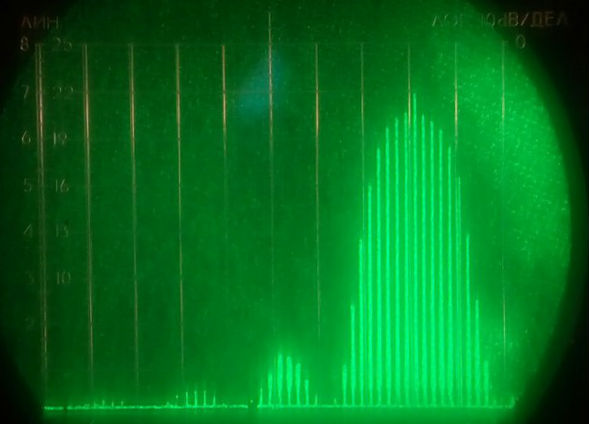
\includegraphics[height=4cm]{B03.jpg} 
   \caption{$f_{\text{повт}} = 2 \text{кГц},~ \tau = 100 \text{мкс},~ f_{0} = 40 \text{кГц}$} 
   \label{fig.b03}
   \end{minipage}
   \hfill
   \begin{minipage}[h!]{0.49\linewidth}
   \centering
   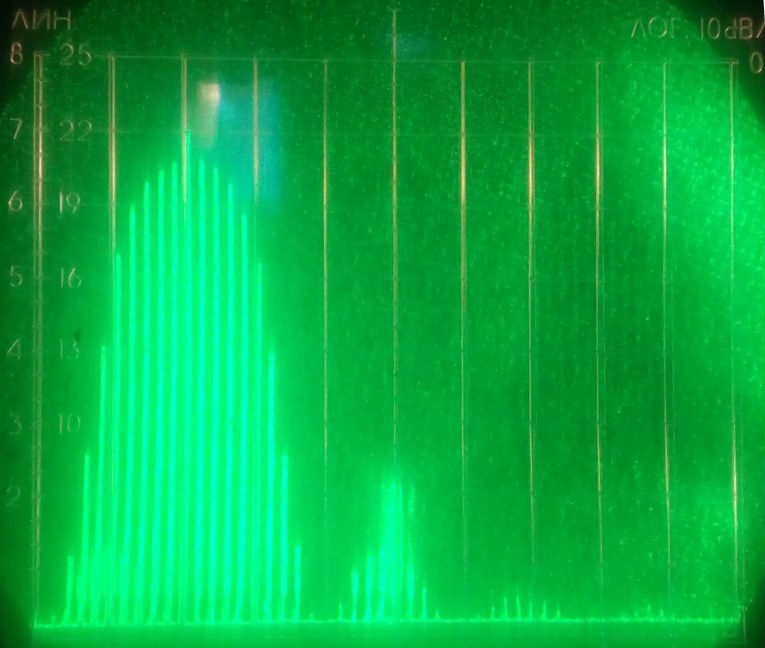
\includegraphics[height=4cm]{B04.jpg} 
   \caption{$f_{\text{повт}} = 2 \text{кГц},~ \tau = 100 \text{мкс},~ f_{0} = 10 \text{кГц}$} 
   \label{fig.b04}
   \end{minipage}  
   \end{figure}

   \begin{table} 
   \begin{center}
   \caption{Зависимость $\delta \nu(\nu_0)$}
   \begin{tabular}{|*{3}{c|}}
   \hline 
   $\nu_0$, кГц & $\delta \nu$, кГц & $\sigma_{\delta \nu}$, кГц\\ \hline 
   1 & 1.0 & 0.1 \\ \hline 
   2 & 2.0 & 0.2 \\ \hline 
   3 & 2.5 & 0.1 \\ \hline 
   4 & 5.0 & 0.5 \\ \hline 
   5 & 5.0 & 0.6 \\ \hline 
   6 & 5.7 & 0.5 \\ \hline 
   7 & 6.7 & 0.7 \\ \hline 
   8 & 7.5 & 0.8 \\ \hline 
   \end{tabular}
   \end{center} 
   \end{table} 

   \begin{figure}[h!]
   \centering
   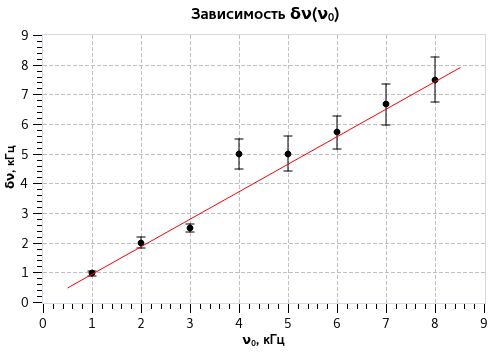
\includegraphics[width=10cm]{fig10.png} 
   \caption{Зависимость $\delta \nu(\nu_0)$} 
   \label{fig.10} 
   \end{figure}

   
\end{document}
